\documentclass[11pt]{article}

% ----------------------------------------------------------------------------
% P1AM Heater / Power-Supply Control System — Architecture Report
% Build:  pdflatex SYSTEM_ARCHITECTURE.tex   (run twice for the ToC/refs)
% Standard packages only (article, geometry, booktabs, hyperref, listings,
% xcolor, longtable, tikz) so it compiles on any full TeX Live install.
% ----------------------------------------------------------------------------

\usepackage[margin=1in]{geometry}
\usepackage{booktabs}
\usepackage{longtable}
\usepackage{xcolor}
\usepackage{listings}
\usepackage{tikz}
\usetikzlibrary{arrows.meta,positioning,fit,backgrounds}
\usepackage[hidelinks]{hyperref}
\usepackage{enumitem}

\definecolor{codebg}{RGB}{245,246,248}
\definecolor{accent}{RGB}{15,90,140}
\lstset{
  basicstyle=\ttfamily\small, backgroundcolor=\color{codebg},
  frame=single, rulecolor=\color{lightgray}, breaklines=true,
  columns=fullflexible, keepspaces=true, showstringspaces=false,
}
\newcommand{\code}[1]{\texttt{#1}}

\title{\textbf{P1AM Heater \& Power-Supply Control System}\\[2pt]
\large Architecture Reference}
\author{Bench SCADA --- \code{src/p1am\_control\_system}}
\date{Generated \today}

\begin{document}
\maketitle
\begin{abstract}
\noindent This report describes the structure of the P1AM bench control system: a
Raspberry\,Pi--hosted SCADA/HMI driving a Facts~Engineering P1AM-100 PLC that runs
a resistive crucible heater (to $\sim$1200\,\textdegree C) under closed-loop
on/off temperature control, plus a programmable power-supply channel. It covers
the hardware stack, the PLC firmware, the FastAPI/Modbus backend, the React HMI,
the safety architecture, the data/historian path, deployment, and the current
engineering findings on thermocouple noise. It is intended as the single
orienting document for anyone operating, extending, or troubleshooting the system.
\end{abstract}

\tableofcontents
\bigskip
\hrule

% ============================================================================
\section{System overview}
% ============================================================================
The system is a three-tier bench SCADA:

\begin{enumerate}[nosep]
  \item \textbf{PLC (real-time I/O + control primitives).} A P1AM-100 (SAMD21
  microcontroller) runs a 10\,Hz scan loop, exposes a 32-channel \emph{tag broker}
  and four PID blocks over \textbf{Modbus TCP}, drives the thermocouple and analog
  I/O cards, and switches the heater relay.
  \item \textbf{Backend (supervisory control + data).} A Python FastAPI/uvicorn
  service on the Raspberry\,Pi polls the PLC at 10\,Hz over Modbus, runs the
  supervisory \emph{temperature} and \emph{power-supply} controllers (state
  machines + control law + safety), applies a thermocouple deglitch filter,
  logs to a SQLite historian, and streams telemetry to the HMI over a WebSocket.
  \item \textbf{HMI (operator interface).} A React/Vite single-page app served on
  the Pi, showing live trends, controls, alarms, a data-explorer analysis suite,
  and a link-diagnostics feed.
\end{enumerate}

\begin{figure}[h]
\centering
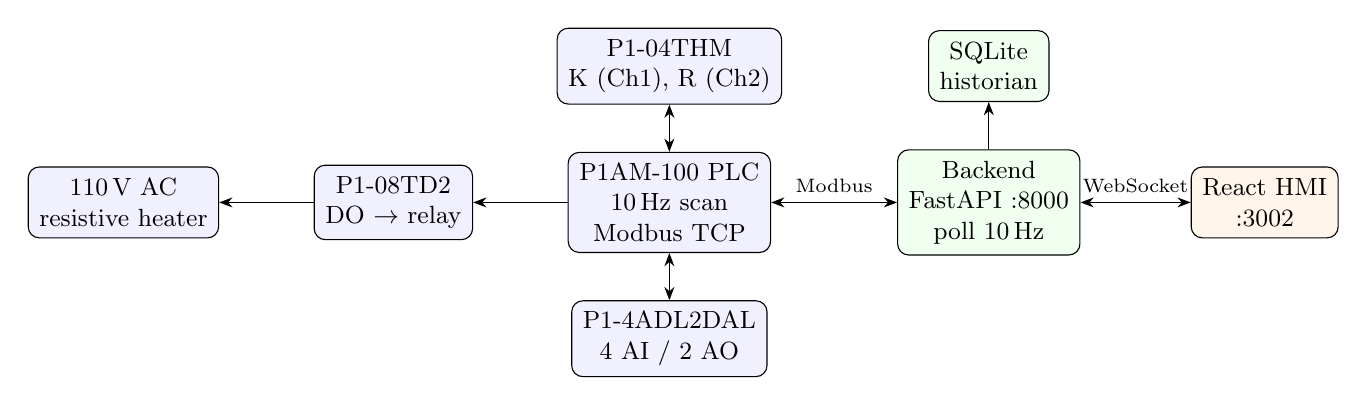
\begin{tikzpicture}[
  node distance=6mm and 12mm, >={Stealth[]},
  box/.style={draw, rounded corners, align=center, minimum height=9mm, inner sep=4pt, font=\small},
  hw/.style={box, fill=blue!6}, sw/.style={box, fill=green!6}, ui/.style={box, fill=orange!8},
]
\node[hw] (heater) {110\,V AC\\resistive heater};
\node[hw, right=of heater] (relay) {P1-08TD2\\DO $\rightarrow$ relay};
\node[hw, right=of relay] (plc) {P1AM-100 PLC\\10\,Hz scan\\Modbus TCP};
\node[hw, above=of plc] (thm) {P1-04THM\\K (Ch1), R (Ch2)};
\node[hw, below=of plc] (adl) {P1-4ADL2DAL\\4 AI / 2 AO};
\node[sw, right=16mm of plc] (be) {Backend\\FastAPI :8000\\poll 10\,Hz};
\node[sw, above=of be] (hist) {SQLite\\historian};
\node[ui, right=14mm of be] (hmi) {React HMI\\:3002};
\draw[->] (relay) -- (heater);
\draw[->] (plc) -- (relay);
\draw[<->] (thm) -- (plc);
\draw[<->] (adl) -- (plc);
\draw[<->] (plc) -- node[above,font=\scriptsize]{Modbus} (be);
\draw[->] (be) -- (hist);
\draw[<->] (be) -- node[above,font=\scriptsize]{WebSocket} (hmi);
\end{tikzpicture}
\caption{End-to-end signal path. The thermocouples close the temperature loop
through the PLC and the backend's supervisory controller.}
\end{figure}

\paragraph{Repository location.} Everything lives under
\code{src/p1am\_control\_system/}: \code{firmware/} (PLC Arduino sketch),
\code{backend/} (Python service), \code{frontend/} (React HMI), \code{deploy/}
(systemd units + install scripts), \code{docs/} (this report), and the bench
runbooks (\code{PI\_BRINGUP.md}, \code{BENCH\_HANDOFF.md}, \code{USER\_MANUAL.md}).

% ============================================================================
\section{Hardware}
% ============================================================================
\begin{longtable}{@{}p{3.4cm} p{4.2cm} p{6.3cm}@{}}
\toprule
\textbf{Component} & \textbf{Part} & \textbf{Role} \\ \midrule
\endhead
Controller       & Raspberry\,Pi 5 (Debian 13 ``trixie'', aarch64) & Hosts the backend + HMI; wired to the PLC on a private subnet. \\
PLC CPU          & P1AM-100 (SAMD21G18A) + W5500 Ethernet & 10\,Hz scan loop; Modbus TCP server at \code{192.168.1.100:502}. \\
Thermocouple I/O & P1-04THM & 4-channel TC module. Ch\,1 = Type-K $\rightarrow$ \code{TAG\_0}; Ch\,2 = Type-R $\rightarrow$ \code{TAG\_1}. Range $0$--$1400$\,\textdegree C, output in \textdegree C. \\
Analog I/O       & P1-4ADL2DAL-1 & 4 analog inputs, 2 analog outputs; also surfaces raw $0$--$5$\,V diagnostic channels. \\
Digital output   & P1-08TD2 & 24\,V DO $\rightarrow$ external relay $\rightarrow$ 110\,V AC resistive heater. \\
Heater           & Resistive element in a refractory-lined crucible & The controlled plant; large thermal mass, target $\sim$1200\,\textdegree C. \\
\bottomrule
\end{longtable}

\noindent The Pi's \code{eth0} is a static \code{192.168.1.50/24} (no gateway) on
the PLC subnet; the PLC answers Modbus at \code{192.168.1.100:502}.

% ============================================================================
\section{Tag broker, register map, and coils}
% ============================================================================
The firmware exposes 32 float \emph{tags} (\code{TAG\_0}\,\ldots\,\code{TAG\_31})
plus routing/PID/interlock configuration, all as Modbus holding registers. The
canonical contract lives in \code{backend/hardware.py} and mirrors
\code{firmware/README.md}.

\begin{longtable}{@{}l l p{7.7cm}@{}}
\toprule
\textbf{Register base} & \textbf{Layout} & \textbf{Meaning} \\ \midrule
\endhead
\code{0}   & \code{TAG\_i} at (\code{2i}, \code{2i+1}) & Tag values, little-endian 32-bit float. \\
\code{100} & channel $\rightarrow$ tag id & Input routing (slots 0--3 TC, 4--5 AI). \\
\code{110} & channel $\rightarrow$ tag id & Output routing (slots 0--1 AO). \\
\code{200} & 4 PIDs $\times$ 10 regs & PID config; setpoint at \code{+2/+3}. \\
\code{300} & 32 tags $\times$ 8 regs & Four-limit interlocks (lolo/low/high/hihi). \\
\bottomrule
\end{longtable}

\begin{longtable}{@{}c l p{8.4cm}@{}}
\toprule
\textbf{Coil} & \textbf{Name} & \textbf{Effect} \\ \midrule
\endhead
\code{0} & \code{SAVE\_TO\_FLASH} & Persist current config to EEPROM/flash. \\
\code{1} & \code{ESTOP\_RESET}    & Clear the latched E-stop (operator re-arm required). \\
\code{2} & \code{HEATER\_RELAY}   & Heater DO: 24\,V $\rightarrow$ relay $\rightarrow$ 110\,V heater. \\
\code{3} & \code{THM\_BURNOUT}    & P1-04THM open-circuit fail direction. \textbf{1 = high-side} (an open reads full scale $\rightarrow$ heater shuts off, \emph{fail-safe}, the default); 0 = low-side (an open reads 0\,\textdegree C, looks cold). Re-asserted every scan so it survives a PLC reboot. \\
\bottomrule
\end{longtable}

\paragraph{Key tag assignments.}
\code{TAG\_0}=Type-K, \code{TAG\_1}=Type-R (active controlling channel),
\code{TAG\_10/11}=analog outputs, \code{TAG\_12/13}=analog inputs,
\code{TAG\_20\,\ldots\,25}=raw $0$--$5$\,V card diagnostics (compare against a
meter at the terminal). Values are percent-of-full-scale where applicable; the
backend scales TC tags to \textdegree C via each channel's \code{full\_scale\_c}.

% ============================================================================
\section{PLC firmware}
% ============================================================================
The Arduino sketch (\code{firmware/}) targets FQBN
\code{P1AM-100:samd:P1AM-100\_native} and is organised as:

\begin{itemize}[nosep]
  \item \code{firmware.ino} --- 10\,Hz scan loop + Modbus TCP server wiring.
  \item \code{SignalBroker} --- the 32-tag broker and routing.
  \item \code{PIDController} --- four PID blocks (available for analog loops).
  \item \code{SafetyInterlock} --- per-tag four-limit interlocks (lolo/low/high/hihi).
  \item \code{P1AMHardware} --- module I/O, including \code{ConfigureThm(bool highSideBurnout)}
        which sets the P1-04THM config byte (0x03 high-side / 0x01 low-side); the
        firmware reads coil~3 each scan and reconfigures on change.
  \item \code{StorageManager} --- EEPROM/FlashStorage-backed config persistence.
\end{itemize}

\noindent \textbf{Flashing caveat:} use the \code{P1AM-100\_native} FQBN only ---
the generic Arduino-Zero FQBN bricks the unit. A 1200-bps bootloader touch drops
the USB CDC off the bus; if a flash reports ``no device on \code{/dev/ttyACM0}''
the Pi's USB must re-enumerate (reboot) before retrying. Build/flash helpers:
\code{run\_pi.sh fw-build|fw-flash}.

% ============================================================================
\section{Backend service}
% ============================================================================
FastAPI/uvicorn on \code{127.0.0.1:8000}. The scan/control path is:

\begin{lstlisting}
poll_runtime  ->  modbus_client (read tags)  ->  thermocouple_filter (deglitch)
              ->  TemperatureController.tick() / PowerSupplyController
              ->  write heater relay coil  +  historian log  +  WebSocket broadcast
\end{lstlisting}

\paragraph{Notable modules.}
\code{poll\_runtime.py} (10\,Hz scan loop), \code{modbus\_client.py} +
\code{modbus\_codec.py} (Modbus I/O), \code{plc\_factory.py} /
\code{simulator\_client.py} (real vs. simulated PLC; \code{PLC\_DRIVER=modbus} for
hardware), \code{temperature\_controller.py} + \code{temperature\_integration.py}
(control + PLC wiring + REST), \code{power\_supply*.py} (the power-supply channel),
\code{safety\_state\_machine.py} (shared safety base --- see \S\ref{sec:safety}),
\code{thermocouple\_filter.py} (deglitch --- \S\ref{sec:deglitch}),
\code{historian.py} + \code{data\_capture.py} (SQLite logging + retention),
\code{data\_explorer\_*.py} (offline analysis suite), \code{config\_store.py}
(durable settings recalled at boot), \code{auth\_config.py} (API auth;
\code{P1AM\_DEV\_NO\_AUTH=1} disables it for bench use).

\paragraph{Selected REST + stream endpoints.}
\code{GET /api/snapshot} (full frame), \code{GET /api/temperature/status|config},
\code{POST /api/temperature/permissive} (Start/Stop; on \emph{off} it de-energizes
the relay \emph{immediately}), \code{POST /api/temperature/setpoint},
\code{POST /api/temperature/tc\_type} (K$\leftrightarrow$R),
\code{POST /api/temperature/burnout\_mode}, \code{POST /api/temperature/acknowledge\_trip},
\code{GET /api/trends} (historian query with server-side decimation across the
whole window), and the telemetry WebSocket the HMI subscribes to.

% ============================================================================
\section{Temperature control law}
% ============================================================================
The heater uses \textbf{on/off (bang-bang) hysteresis} around the setpoint --- it
is a relay, not an analog output:

\begin{itemize}[nosep]
  \item Relay \textbf{ON} when measured $\le$ setpoint $-$ \code{deadband\_c}.
  \item Relay \textbf{OFF} when measured $\ge$ setpoint $+$ \code{deadband\_c}.
  \item Inside the band the relay \textbf{holds} its prior state (no chatter).
  \item \textbf{Anti-short-cycle:} after a switch the relay is held for at least
        \code{min\_on\_time\_s} / \code{min\_off\_time\_s} before the opposite
        demand is honoured (enforced only when a monotonic clock is supplied).
\end{itemize}

\noindent Current config (\code{Type-R} controlling): full scale $1400$\,\textdegree C,
setpoint range $0$--$1400$, \code{deadband\_c}$=5$, HH limit $=1400$,
min on/off $=0$\,s. The control feedback is the \emph{filtered} active-TC value;
both channels are always scaled and filtered so a channel switch lands on an
already-warm filter.

% ============================================================================
\section{Safety architecture}\label{sec:safety}
% ============================================================================
\code{TemperatureController} and \code{PowerSupplyController} both extend
\code{SafetyStateMachine[StateT]}, which owns the identical scaffolding:

\begin{description}[nosep,leftmargin=1.4cm,style=nextline]
  \item[States] IDLE $\rightarrow$ ARMED (permissive on) $\rightarrow$ RUNNING
  (setpoint applied) $\rightarrow$ TRIPPED. Permissive off returns to IDLE and
  clears the setpoint.
  \item[Force-off invariant] \code{\_should\_force\_actuator\_off()} is true in
  \emph{every} state except genuine RUNNING (armed, no E-stop, no trip). The
  heater relay is force-held \textbf{off} in IDLE/ARMED/TRIPPED/E-stop/any-trip.
  This is why seeding a setpoint at boot can never energize the heater.
  \item[E-stop] A one-way latch: forces IDLE, disarms, drops the setpoint, and
  refuses re-arm/setpoints until explicitly cleared.
  \item[Trips] Latch until \code{acknowledge\_trip()}. Trip types below.
\end{description}

\paragraph{Temperature trips.}
\begin{itemize}[nosep]
  \item \textbf{HH\_TEMP} --- high-high cutoff, latched the instant \emph{either}
  thermocouple reaches \code{hh\_limit\_c} (a dead controlling sensor cannot mask
  a real over-temperature).
  \item \textbf{TC\_DISAGREE} --- debounced cross-check: while RUNNING, if the
  controlling TC reads essentially cold ($<100$\,\textdegree C) while the other
  reads clearly hot ($\ge 200$\,\textdegree C) for several consecutive scans, the
  controlling sensor is lying and the heater trips.
  \item \textbf{TC\_FAULT} --- a non-finite/garbage feedback while RUNNING (an open
  that reads NaN) trips rather than coercing to ``cold''.
\end{itemize}

\paragraph{Defense-in-depth.} A service-level E-stop interlock in
\code{\_write\_relay} forces the relay off independently of the controller latch,
retries a failed de-energize, and raises a comms alarm if it still fails. A
\textbf{Stop} routes through \code{TemperatureService.set\_permissive(False)},
which commands the relay off \emph{within the request} (not on the next scan). The
HMI Stop button is deliberately \emph{unconditional} --- never gated behind a
confirmation dialog, which a kiosk browser can suppress.

% ============================================================================
\section{Thermocouple deglitch filter}\label{sec:deglitch}
% ============================================================================
An open/failing thermocouple is driven to a burnout \emph{rail} (0\,\textdegree C
low-side or full-scale high-side) --- a perfectly finite number that the
non-finite \code{TC\_FAULT} check never catches, and that the control law would
believe. \code{ThermocoupleDeglitchFilter} sits between the tag$\rightarrow$\textdegree C
conversion and the controller and:

\begin{itemize}[nosep]
  \item accepts plausible readings unchanged;
  \item \textbf{rejects} an implausible jump toward either rail, or any
  non-physical single-scan step, \textbf{holding the last-good} value so the
  control law never acts on a glitch;
  \item if the fault \emph{persists} past \code{hold\_timeout\_s} ($15$\,s),
  declares a hard fault so the caller trips the heater (holding a stale value
  forever would let it heat blind).
\end{itemize}

\noindent This protects the \emph{control} path and the filtered status values.
The \emph{raw} tag stream (logged to the historian and drawn on the multi-tag
trend) is unfiltered by design, so the HMI trends additionally bridge isolated
dropped-read zeros for display (\S\ref{sec:findings}).

% ============================================================================
\section{HMI (React frontend)}
% ============================================================================
Vite dev/preview on \code{:3002}, proxying \code{/api} + the WebSocket to the
backend. Tabs: \emph{Trends \& Monitors}, \emph{Data Explorer}, \emph{PID \& Mass
Flow}, \emph{Signal Routing}, \emph{Tuning \& MPC}, \emph{Events \& Alarms},
\emph{Ladder}, \emph{Plant Hierarchy}, \emph{Power Supply}, \emph{Heater
Controls}, \emph{Signal Diagnostics}.

\paragraph{Trends.} Bespoke SVG charts (no chart library) with a shared
pan/zoom/pause/drag-to-zoom viewport model, a hover crosshair + value tooltip on
every plot, PNG/SVG/CSV snapshot export, and time windows up to 24\,h backed by
historian backfill with server-side decimation. Panels are drag-to-reorder and
vertically resizable (arrangement persisted per tab).

\paragraph{Live-link diagnostics.} A collapsible bar shown on \emph{every} tab:
LIVE/STALE/OFFLINE, effective arrival rate (Hz), staleness, and the K\,/\,R\,/\,$\Delta$\,/\,relay
summary; it expands to a scrollable feed of the most recent \emph{raw} PLC tag
values (a lone 0 is a likely dropped read), with a copy-to-share button.

% ============================================================================
\section{Data \& historian}
% ============================================================================
SQLite \code{dcs\_scada.db}: a long-format \code{taglog} (tag name, timestamp,
value; \textbf{naive-UTC} timestamps) and an \code{eventlog}. Capture is
\textbf{decimated} (a configurable throttle interval), \emph{not} the full 10\,Hz
scan --- so historian sample spacing is on the order of seconds, and dropout
\emph{rates} should be read as fractions of logged samples, not per-scan. A
size-based retention loop purges the oldest rows above a byte cap ($\sim$2\,GiB).
\code{GET /api/trends} decimates server-side so a multi-hour window returns points
spanning the whole range rather than only the newest slice.

% ============================================================================
\section{Deployment \& remote access}
% ============================================================================
Two systemd units (\code{Restart=always}): \code{p1am-backend} (uvicorn) and
\code{p1am-frontend} (\code{vite preview}, rebuilds on start). Installed via
\code{deploy/install-services.sh}; the desktop launcher (\code{launch-hmi.sh})
prefers the raw \code{/usr/lib/chromium/chromium} binary (the \code{/usr/bin}
wrapper injects a flag that aborts launch). Remote access: \textbf{Raspberry\,Pi
Connect} (screen sharing over Wayland/labwc), \textbf{wayvnc over Tailscale}
(bound to \code{100.108.70.33:5900}, reachable only by authenticated Tailscale
peers), and \textbf{SSH}.

% ============================================================================
\section{Engineering findings: thermocouple noise}\label{sec:findings}
% ============================================================================
Investigation of the ``dips to zero'' on the R trend established:

\begin{itemize}[nosep]
  \item The zeros are \textbf{real dropped reads in the acquired data}, not a
  plotting artifact --- but they are \textbf{rare and episodic}, not a constant
  rate (the bulk of logged zeros are long \emph{sustained} runs from
  system-off / a sensor not yet in the vessel).
  \item They are \textbf{high-temperature gated}: a burst measured $\sim$6\,\%
  dropouts on R at $\sim$1180\,\textdegree C (near setpoint), while a controlled
  capture at $\sim$800\,\textdegree C saw \emph{zero} over $\sim$1700 raw samples.
  Heater-ON periods roughly double the dropout rate vs. heater-OFF.
  \item \textbf{Mechanism:} above $\sim$1000--1100\,\textdegree C the refractory
  becomes mildly conductive, opening a leakage/ground path that couples the AC
  heater's noise onto the low-output ($\sim$10\,\textmu V/\textdegree C), sleeved
  Type-R thermocouple. It worsens toward 1200\,\textdegree C+.
  \item \textbf{Recommended fix:} an isolated TC transmitter/signal conditioner on
  R (galvanic isolation + filtering) plus single-point grounding of the TC
  shield/sheath. Software already mitigates: the deglitch filter holds last-good
  through the glitches and the trends bridge them for display.
  \item \textbf{Note:} earlier readings of K near ambient were K \emph{not yet
  installed in the vessel} (sitting on the bench), not a K termination fault.
\end{itemize}

\vfill
\begin{center}\small\itshape
This report reflects the system as built at generation time; verify port/path/
config specifics against the code and \code{/api/temperature/config} before
relying on them operationally.
\end{center}

\end{document}
